\documentclass{article}
\usepackage[a4paper, total={6in, 8in}]{geometry}
\usepackage{algorithm}
\usepackage{algpseudocode}
\usepackage{float}
\usepackage{hyperref}
\usepackage{graphicx}
\graphicspath{ {images/} }

\usepackage[utf8]{inputenc}
\usepackage[english]{babel}
\usepackage{amsthm}
\theoremstyle{definition}
\newtheorem{definition}{Definition}[section]
\usepackage{forest}

\usepackage{listings}
\usepackage{color}
\definecolor{folderbg}{RGB}{124,166,198}
\definecolor{folderborder}{RGB}{110,144,169}
\definecolor{dkgreen}{rgb}{0,0.6,0}
\definecolor{gray}{rgb}{0.5,0.5,0.5}
\definecolor{mauve}{rgb}{0.58,0,0.82}
\definecolor{lbcolor}{rgb}{0.9,0.9,0.9}

\def\Size{4pt}
\tikzset{
  folder/.pic={
    \filldraw[draw=folderborder,top color=folderbg!50,bottom color=folderbg]
      (-1.05*\Size,0.2\Size+5pt) rectangle ++(.75*\Size,-0.2\Size-5pt);
    \filldraw[draw=folderborder,top color=folderbg!50,bottom color=folderbg]
      (-1.15*\Size,-\Size) rectangle (1.15*\Size,\Size);
  }
}

\lstset{
tabsize=4,
basicstyle=\ttfamily,
backgroundcolor=\color{lbcolor},
showstringspaces=false
}
% \lstset{frame=tb,
%   language=Java,
%   aboveskip=3mm,
%   belowskip=3mm,
%   showstringspaces=false,
%   columns=flexible,
%   basicstyle={\small\ttfamily},
%   numbers=none,
%   numberstyle=\tiny\color{gray},
%   keywordstyle=\color{blue},
%   commentstyle=\color{dkgreen},
%   stringstyle=\color{mauve},
%   breaklines=true,
%   breakatwhitespace=true,
%   tabsize=3
% }


\begin{document}

\begin{titlepage}
	\newcommand{\HRule}{\rule{\linewidth}{0.5mm}}
	\center % Centre everything on the page
	\textsc{\LARGE Iowa State University}\\[1.5cm]
	\HRule\\[0.4cm]
	{\huge\bfseries R2U2: User Guide}\\[0.4cm]
	\HRule\\[1.5cm]
	\vfill
	\textbf{Summary}: This document contains all the information a user would need in order to use the open source R2U2 runtime verification tool. Described within are the tool-flows for the three main implementations of R2U2: Python, C, and VHDL.
	\vfill
	\textbf{Investigators:} Dr.s Kristen Yvonne Rozier, Phillip H. Jones, Joseph Zambreno
	
	\textbf{Graduate Students:} Pei Zhang, Brian Kempa, Matthew Cauwels, Balaji Sivasubramanian
	\vfill
	{\large\today}
	\vfill
\end{titlepage}


\tableofcontents
\clearpage

\section{Introduction}
R2U2 - a \textbf{Realizable}, \textbf{Responsive}, \textbf{Unobtrusive} \textbf{Unit} - is a state-of-the-art streaming runtime verification monitor.  

\subsection{R2U2 Architecture Overview}

\subsection{Accessing the GitHub Repository}


\clearpage

\section{R2U2 Software Implementation in C++}
The C++ version of R2U2 can be executed offline, as a trace and/or MLTL formula validation tool, or online, as a streaming runtime monitor. The offline version serves as a way for a user to validate an MLTL formula over a trace and it helps developer's perform regression testing across pre-validated traces \& formulae. The online version executes a streaming runtime monitor, which can execute on either an embedded processor or a personal computer. Similar to the R2U2-C version, the embedded sensor's data must be saved into a file structure that R2U2 accesses. Additionally, the sensor data must be pre-processed into Boolean atomics before R2U2-C++ can reason over them.

\subsection{Getting Started}
The C++ implementation of R2U2 runs from a UNIX based command line interface (CLI). Additionally, there are several types of files users must use:
\begin{itemize}
	\item \textbf{Assembly File:} The \textit{.ftasm} file that stores the assembly code for the MLTL formula. The details and an example of this 
	\item \textbf{Trace File:} The sensor information from either an offline or online trace need to be stored into one or more \textit{.log} files. The details for how to modify the \textit{MTL.cpp} file for the user specific \textit{.log} files, how to format the \textit{.log} files, and examples of each will be given in Section \ref{Cpp_Sensor}.
	\end{itemize}
	

\subsection{File Formats}
Note that user must provide the \textit{.ftasm} file and one or more \textit{.log} files to run this version of R2U2. The \textit{.ftasm} assembly file specifies the temporal logic formulas over which the atomic propositions are reasoned over. The \textit{.log} files are the atomic sensor traces that are being reasoned over.

\subsubsection{Assembly File:}
\label{AssemblyFile}
Like any other assembly file, this file is a list of single command instructions that R2U2 will execute, in order. An example of a R2U2 compatible Assembly File can be seen in Table \ref{CppFileTable}. Each line contains an instruction, which consists of a label, a command, and one or more variables/labels. The list of assembly commands the C++ version of R2U2 can use is:
\begin{itemize}
	\item \textbf{\textit{load}:} Used to load the atomic from either the Sensor Input File or Atomic Input File. 
	\item \textbf{\textit{not}:} Used to denote the logical \textit{Negation} of an atomic.
	\item \textbf{\textit{and}:} Used to denote the logical \textit{AND} of two atomics.
	\item \textbf{\textit{until}:} Used to denote the \textit{Until} temporal logic function. This function takes in four arguments: the first is the label for the left-side of the \textit{Until}, the second is the right-side, the third is the relative start time, and the fourth is the relative end time.
	\item \textbf{\textit{boxbox}:} Used to denote the \textit{Global} temporal logic function. Assumes that the time bound starts at zero. First argument is the label (either atomic or instruction), the second is the relative end time of the function.
	\item \textbf{\textit{boxdot}:} Used to denote the \textit{Global} temporal logic function. First argument is the label (either atomic or instruction), the second is the relative start time of the function, and the third is the relative end time of the function.
	\item \textbf{\textit{end}:} Used to denote the end of the assembly file. This command must be at the end of the Assembly File and its argument must be the second-to-last label.
\end{itemize}

\begin{table}[H]
	\caption{Examples of the format for the \textit{.ftasm} file.
	\label{CppFileTable}}
	\begin{center}
	\begin{tabular}{l | l}
		\hline
		\hline
		\textbf{File Type} & \textbf{Assembly File}\\
		\hline
		line 1 & load\_ft a000\\
		line 2 & load\_ft a001\\
		line 3 & not s000\\
		line 4 & not s001\\
		line 5 & and s002 s003\\
		line 6 & and s000 s001\\
		line 7 & not s005\\
		line 8 & until s006 s005 0 3\\
		line 9 & boxbox s007 3\\
		line 10 & end s008\\
		\hline
		\hline
	\end{tabular}
	\end{center}
\end{table}

\subsubsection{Trace File Formats}
\label{Cpp_Sensor}
The trace information must be passed to R2U2-C++ via \textit{.log} files. These \textit{.log} files must be specified in the \textit{MTL.cpp} file. How this is done as well as the formatting for the input files will be described in this section.

\subparagraph{Modifying the \textit{MTL.cpp}}
\label{Mod_MTL}
Within the \textbf{R2U2\_SW/R2U2\_Cpp/src} directory is the \textit{MTL.cpp} file. This file must be modified in order to interface R2U2 with all of the \textit{.log} files R2U2 will read. A screenshot of the code that must be modified can be seen in Fig. \ref{fig:r2u2cppMod}. 

\begin{figure}[H]
	\begin{center}
	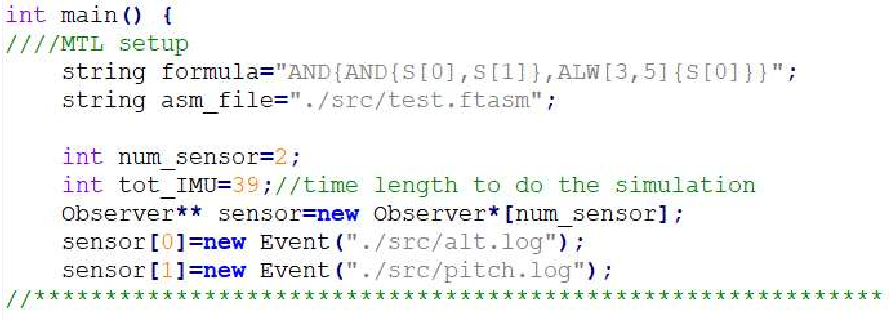
\includegraphics[scale=0.5]{fig/r2u2_cpp_MTL.pdf}
	\caption{A screenshot of the user modified code in \textit{MTL.cpp}. In this example, there are two sensor traces: \textit{alt.log} and \textit{pitch.log}.
	\label{fig:r2u2cppMod}} 
	\end{center}
\end{figure} 

Several values must be tailored to the specific project, namely: \textbf{num\_sensor} and \textbf{tot\_IMU} must be set to the specific number of \textit{.log} files for the application as well as how many time stamps long R2U2 will execute. For each \textit{.log} file, the \textit{.log} file's location must be specified within the \textbf{sensor} array.

\subparagraph{Atomic Input File:}
\label{Cpp_InputFile}
The values of the atomic input file must be Booleans, i.e., a $0$ or $1$. Thus, the sensor value must be pre-processed into a Boolean value via a comparison operator. An example of the format can be seen in Table \ref{CppTraceTable}.

\begin{table}[H]
	\caption{Examples of the format for the Trace Files.
	\label{CppTraceTable}}
	\begin{center}
	\begin{tabular}{l | cc}
		\hline
		\hline
		\textbf{File Type} & \multicolumn{2}{c}{\textbf{Atomic Input File}}\\
		\hline
		Line \# & Atomic & Time\\
		\hline
		line 1 & 0 & 0\\
		line 2 & 0 & 1\\
		line 3 & 1 & 2\\
		line 4 & 0 & 3\\
		line 5 & 1 & 4\\
		$\vdots$ & $\vdots$ & $\vdots$\\
		\hline
		\hline
	\end{tabular}
	\end{center}
\end{table}

\subsection{CLI Overview}
\begin{enumerate}
%***** #1	
	\item Navigate to the \textbf{R2U2\_SW/R2U2\_Cpp/src} directory via:
	\begin{lstlisting}[language=C]
	cd R2U2_Cpp/src
	\end{lstlisting}
	\begin{enumerate}
	%***** #a
		\item For the offline version of R2U2-C++, place the sensor trace files in this directory, following the syntax from Section \ref{Cpp_InputFile}.
		\item For the online version of R2U2-C++, ?
	\end{enumerate}
%***** #2
	\item Modify \textit{MTL.cpp} sensor input information. The quantity of sensors and the files the sensor information will be read from must be modified. See Section \ref{Cpp_Sensor} for details.
%***** #3
	\item Navigate to the \textbf{R2U2\_SW/R2U2\_Cpp} directory via:
	\begin{lstlisting}[language=C]
	cd ../
	\end{lstlisting}
%***** #4
	\item Compile R2U2-C++ via:
	\begin{lstlisting}[language=C]
	make
	\end{lstlisting}
%***** #5
	\item To launch R2U2-C++, exectute:
	\begin{lstlisting}[language=C]
	./build/app/main
	\end{lstlisting}
\end{enumerate}

\clearpage

\section{R2U2 Software Implementation in C Programming}
The C version of R2U2 has two modes of operation: an offline mode and an online mode. The offline mode functions similar to the Python implementation of R2U2: it provides an offline verification of a trace or it can be used to validate an MLTL formula over a trace. Additionally, this offline mode allows developers to perform regression testing over a variety of benchmark traces \& formulas to make sure updates did not break the tool. The online version is intended to be versatile; it can be run either on an embedded platform or a personal computer. Note that this online version requires the sensor values R2U2 is reasoning over to be continuously written into a file structure, which means that the embedded platform must support writing to a file.

\subsection{Getting Started}
Note that the following must be installed to use the C implementation of R2U2:
\begin{itemize}
	\item \textbf{Python:} Version 3.6 (or greater)
	\item \textbf{Python Packages:} ply
	\item \textbf{Unix Packages:} pkg-config, fftw3
\end{itemize}
\subparagraph{R2U2 Tool-chain Flow:} Figure \ref{fig:r2u2cflow} shows the flow of the C version of R2U2. To use this version of R2U2, the user needs to supply R2U2 with a trace file (\textit{.trc}) and an MLTL formula. The user starts by converting the MLTL formula into an Assembly File (\textit{.ftasm}). Within this step, the SCQ size (amount of memory required for R2U2's instruction sequence) is determined and stored in a \textit{.ftscq} file. The second step is to take this \textit{.ftasm} assembly file and convert it into a Binary Instruction (\textit{.ftm}) and an Binary Instruction Interval (\textit{.fti}). Lastly, the user specifies their \textit{.ftm}, \textit{.fti}, \textit{.ftscq}, and their own \textit{.trc} file to R2U2, via a UNIX command line. R2U2 compiles this information and begins its online or offline execution. The results of R2U2 are displayed through the command terminal and logged into a \textit{.log} file within the \textbf{R2U2\_SW/R2U2\_C} directory.

\begin{figure}[H]
	\begin{center}
	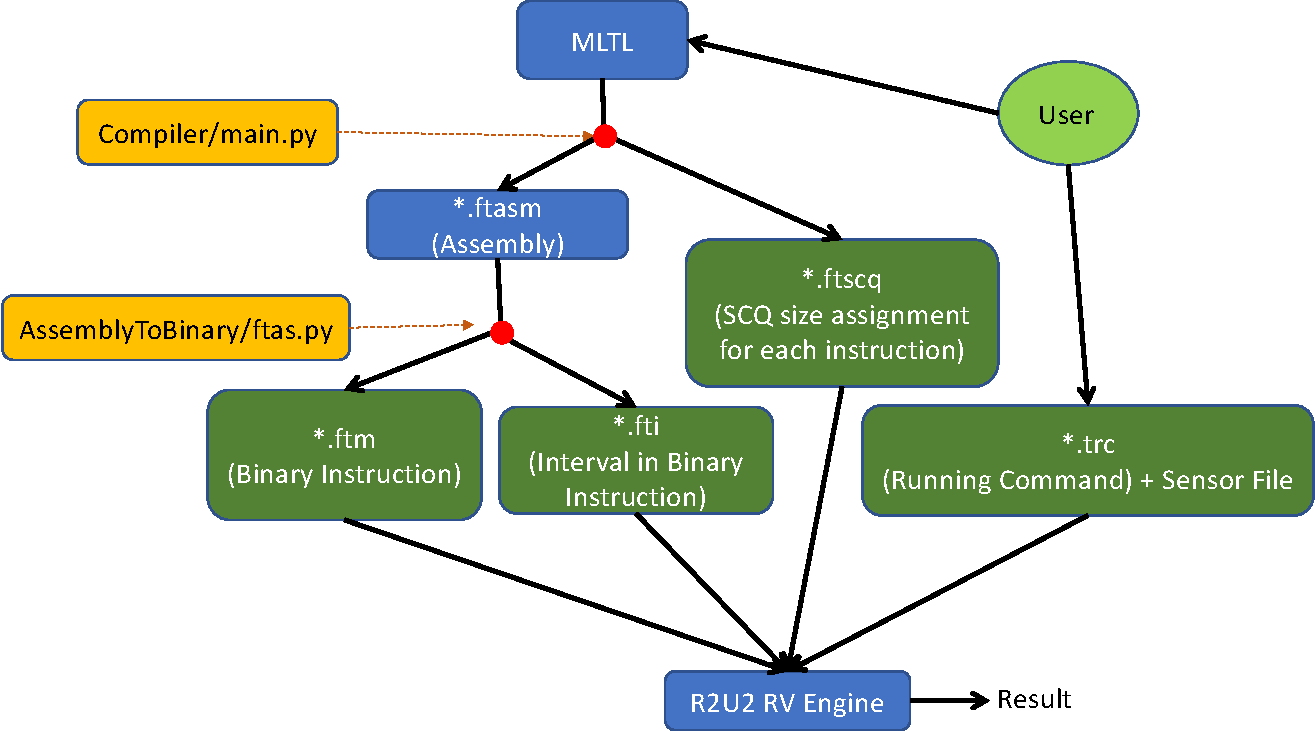
\includegraphics[scale=0.5]{fig/r2u2_c_flow.pdf}
	\caption{Flow of how the C version of R2U2 is compiled and deployed. 
	\label{fig:r2u2cflow}} 
	\end{center}
\end{figure}

The C version of R2U2 must be executed from a UNIX based command line interface (CLI). Described below are the file types that the user must supply to run R2U2:
\begin{itemize}
	\item \textbf{MLTL Formula:} This is the MLTL formula R2U2 will reason over. This formula can be either directly entered into the CLI or saved into the \textit{main.py} file within the \textbf{/tools/Compiler/} directory of R2U2. More detail into the syntax of the MLTL formula will be described in Section \ref{mltlFormula}. 
	\item \textbf{Trace File:} This file contains the sensor values R2U2 will reason over. Note that there will be two different formats for this file depending on whether R2U2 will be run offline or online. More detail into the two file formats, the syntax, and how to convert these sensor values into Boolean atomics will be discussed in Section \ref{TraceFile}.
\end{itemize}

\subsection{File Formats}
\label{FileFormats}
This version of R2U2 has two input parameters: an MLTL formula and a trace file. This section describes the syntax \& structure for theses files and how a user would incorporate them into the current R2U2 structure.

\subsubsection{MLTL Formula}
\label{mltlFormula}
The MLTL formula that R2U2 will reason over must be implemented in one of two ways: either written and saved into the \textit{main.py} file (located within the \textbf{tools/Compiler} directory) or entered directly into the CLI when compiling the \textit{.ftasm} assembly file. In either case the syntax for the MLTL formula is identical and can be seen in Table \ref{mltlFormulaTable}. Note that the only difference is how special characters are labeled in the CLI: they must be proceeded with a `` $\setminus$ ''. Additionally, the syntax for the MLTL formulas can be seen in Table \ref{syntaxMLTL}.

\begin{table}[H]
	\caption{An example of an MLTL formula and the syntactical conversion into either the file type or the CLI.}
	\label{mltlFormulaTable}
	\begin{center}
	\begin{tabular}{l | l}
		\hline
		\hline
		\textbf{Type} & \textbf{Formula Format}\\
		\hline
		Expression & $G_{0,3}((a_0\bigwedge a_1)\bigwedge (a_2 \bigwedge s_3))$\\
		\textit{main.py} & MLTL = ``G[0,3]((a0 \& a1) \& (a2 \& a3))''\\
		CLI & G[0,3]((a0$\setminus$\&a1) $\setminus$\&(a2$\setminus$\&a3))\\
		\hline
		\hline
	\end{tabular}
	\end{center}
\end{table}

%\begin{table}[H]
%	\caption{The format for the MLTL operators, which are used to create a single MLTL formula which can either be saved to the \textit{main.py} file or incorporated into the CLI. Note that $E$1 and $E$2 denote that that parameter can be either an expression, to allow for more complex formulas, or a single atomic.}
%	\label{syntaxMLTL}
%
%	\begin{center}
%	\begin{tabular}{l | c | c | c | c | c | c}
%		\hline
%		\hline
%		\textbf{Expression} & \textit{NOT} & \textit{Next} & \textit{Until} & \textit{Global} & \textit{AND} & \textit{OR}\\
%		\hline
%		\textbf{Syntax} & !$E$1 & $XE$1 & $E$1 $U$[$t_i$,$t_f$] $E$2 & $G$[$t_i$,$t_f$] $E$1 & $E$1 \& $E$2& $E$1 $|$ $E$2\\
%		\hline
%		\textbf{Precedence} & 1 & 1 & 2 & 2 & 3 & 3\\
%		\hline
%		\hline
%	\end{tabular}
%	\end{center}
%\end{table}

\begin{table}[H]
	\label{syntaxMLTL}

	\begin{center}
	\begin{tabular}{l | c  }
		\hline
		\hline
		\textbf{Expression} & \textit{Syntax} \\
		\hline
		Negation     & \texttt{!E1} \\
		Conjunction  & \texttt{E1 \& E2}\\
		Disjunction  & \texttt{E1 | E2} \\
		Implication  & \texttt{E1 -> E2} \\
		Equivalence  & \texttt{E1 <-> E2}\\
		\hline
		Globally     & \texttt{G[ti,tf] E1} or \texttt{G[tf] E1} \\
		Future       & \texttt{F[ti,tf] E1} or \texttt{F[tf] E1}\\
		Until        & \texttt{E1 GU[ti,tf] E2} or \texttt{E1 U[tf] E2} \\
		\hline
		Historically & \texttt{H[ti,tf] E1} or \texttt{H[tf] E1} \\
		Once         & \texttt{O[ti,tf] E1} or \texttt{O[tf] E1} \\ 
		Since        & \texttt{E1 S[ti,tf] E2} or \texttt{E1 S[tf] E2} \\
		\hline
		\hline
	\end{tabular}
	\end{center}
\end{table}

\subsubsection{Trace File}
\label{TraceFile}
In addition to the MLTL formulas, users need to supply a time series of sensor data, i.e., a trace file. There are two different formats for this file: one for the offline version and one for the online. Both versions are described in Table \ref{SensorFileTable}.

\begin{table}[H]
	\caption{Examples of the format for the \textit{.trc} Trace Files}
	\label{SensorFileTable}
	\begin{center}
	\begin{tabular}{l | ccc | cccc}
		\hline
		\hline
		\textbf{File Type} & \multicolumn{3}{c|}{\textbf{Offline \textit{.trc} File}} & \multicolumn{4}{c}{\textbf{Online \textit{.trc} File}}\\
		\hline
		Line \# & Sensor 0 & Sensor 1 & $\dots$ & Command & Sensor 0 & Sensor 1 & $\dots$\\
		\hline
		line 1 & 1002 &  9.9 & $\dots$ & \textbf{i} & 1002 &  9.9 & $\dots$\\
		line 2 & 1005 & 10.0 & $\dots$ \\
		line 3 & 1011 &  9.8 & $\dots$ \\
		line 4 & 1015 & 10.4 & $\dots$ \\
		line 5 & $\vdots$ & $\vdots$ & \\
		\hline
		\hline
	\end{tabular}
	\end{center}
\end{table}
Note that the online version's trace file must be written on each time stamp. Additionally, a command structure is introduced in the first column of the online \textit{.trc} file to allow R2U2 to initialize, increment the time stamp, and to terminate execution. The values of these commands are as follows:
\begin{itemize}
	\item \textbf{i = -2:} Terminate the current execution.
	\item \textbf{i = -1:} Reset R2U2 to its initial state.
	\item \textbf{i $\geq$ 0:} The time stamp for R2U2 (starting at i = 0).
\end{itemize}

In addition to providing the trace file, the user must specify how the sensor inputs will be converted into Boolean atomics. The \textbf{at\_checkers\_update} function  within the \textit{at\_conversion.c} file must be modified to perform this conversion. This file is contained within the \textbf{R2U2\_SW/R2U2\_C/src/AT/} directory. Figure \ref{fig:atConversion} shows the \textit{at\_conversion.c} function with an example conversion of $\textit{Sensor 0}<1000$, $\textit{Sensor 0}>950$, $\textit{Sensor 1}>9.5$, and $\textit{Sensor 1}<10.0$.

\begin{figure}[H]
	\begin{center}
		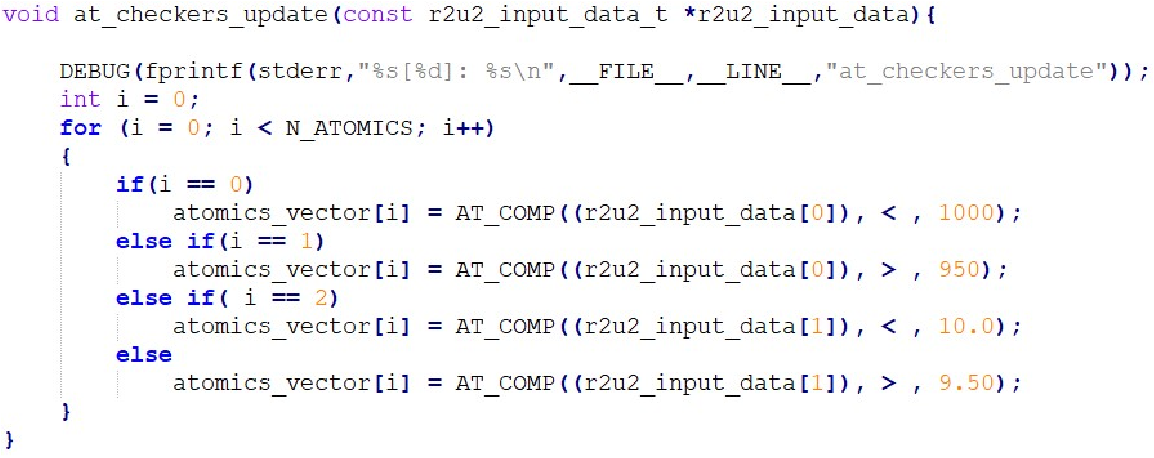
\includegraphics[scale=0.5]{fig/ATconversionScreenshot.pdf}
		\caption{A screenshot of the \textbf{at\_checkers\_update} function within the \textit{at\_conversion.c} file. Note that this function must be modified in order to convert the sensor values into boolean atomics.
		\label{fig:atConversion}}
	\end{center}
\end{figure}

\subsection{Running R2U2 - C Version}
\label{R2U2c}


\subsubsection{Offline Execution Steps}
\label{OfflineC}
\begin{enumerate}
	\item Navigate to the \textbf{../R2U2\_SW/R2U2\_C/} directory
	\item In a UNIX bash terminal, compile the project using the command
	\begin{lstlisting}[language=C]
	make
	\end{lstlisting}
	\item Modify the \textbf{at\_conversion.c} function to convert the sensors into boolean atomics.
	\item Navigate backwards to the \textbf{tools} directory via 
	\begin{lstlisting}[language=C]
	cd ../../tools
	\end{lstlisting}
	\item Next, the \textit{.ftasm} \& the \textit{.ftscq} files must be complied. There are two ways to proceed, depending on how the user wishes to input the MLTL formula:
	\begin{enumerate}
		\item \textbf{main.py:} Execute the command
		\begin{lstlisting}[language=C]		
		python Compiler/main.py
		\end{lstlisting}
		\item \textbf{CLI:} Execute the command
		\begin{lstlisting}[language=C]
		python Compiler/main.py [MLTL Formula]
		\end{lstlisting}
	\end{enumerate}
	\item Compile the \textit{.ftm} \& \textit{.fti} files from the newly generated \textit{.ftasm} using the command:
	\begin{lstlisting}[language=C]
	cat tmp.ftasm | python AssemblyToBinary/ftas.py tmp
	\end{lstlisting}
	\item Navigate back to the \textbf{R2U2\_C} directory via
	\begin{lstlisting}[language=C]
	cd ../R2U2_C
	\end{lstlisting}
	\item Begin R2U2's execution with the following command:
	\begin{lstlisting}[language=C]
	./bin/r2u2 [location of .trc file, from current directory] 
	[location of the .ftm file] [location of the .fti file] 
	[location of the .ftscq file]
	\end{lstlisting}

\end{enumerate}

\subsubsection{Online Execution Steps}
\label{OnlineC}


\clearpage

\section{R2U2 Hardware Implementation in VHDL}
The VHDL version of R2U2 has two modes of operation: an offline mode and an online mode. The offline mode reasons over a logged trace of sensor data, which can be used to validate an MLTL formula over a trace and for regression testing over a variety of benchmark formulas \& traces. Conversely, the online version reads streaming sensor data, which is read directly from a data bus or a custom preprocessing hardware block, and transmits its verdict via UART to a host PC.

\subsection{Getting Started}
Note that this version of R2U2 was designed in Xilinx's Vivado 2017.2. Additionally, the following are needed to compile this version of R2U2
\begin{itemize}
	\item \textbf{Python:} Version 2.6 (or greater) \textbf{and} Version 3.6 (or greater)
	\item \textbf{Packages:} pyserial, ply
\end{itemize}

\subparagraph{R2U2-VHDL Tool-chain Flow:} Figure \ref{fig:r2u2hwFlow} shows the tool-chain flow of the VHDL version of R2U2. To use this version of R2U2, the user needs to supply R2U2 with an MLTL formula and a custom VHDL file for interfacing with a data bus and/or a set of sensors. If the user wishes to use the offline mode, they must also supply a trace of sensor data. The user will start by compiling their MLTL formula into an Assembly File (\textit{.ftasm}). Within this step, the SCQ size (amount of memory required for R2U2's instruction sequence) is determined and stored in a \textit{.ftscq} file. The \textit{.ftasm} must then be compiled into a Binary Instruction (\textit{.ftm}) and a Binary Instruction Interval (\textit{.fti}) file. In parallel, the user must configure R2U2-VHDL's parameters to match those of the desired sensor values. This is done by modifying the \textit{config.py}, \textit{inputs.py}, and the \textit{.ast} file. Additionally, the user must incorporate their own custom hardware for interfacing their current system with R2U2 to run online. This version of R2U2 can also be run offline, i.e., fed a trace of sensor data via UART. 

\begin{figure}[H]
	\begin{center}
	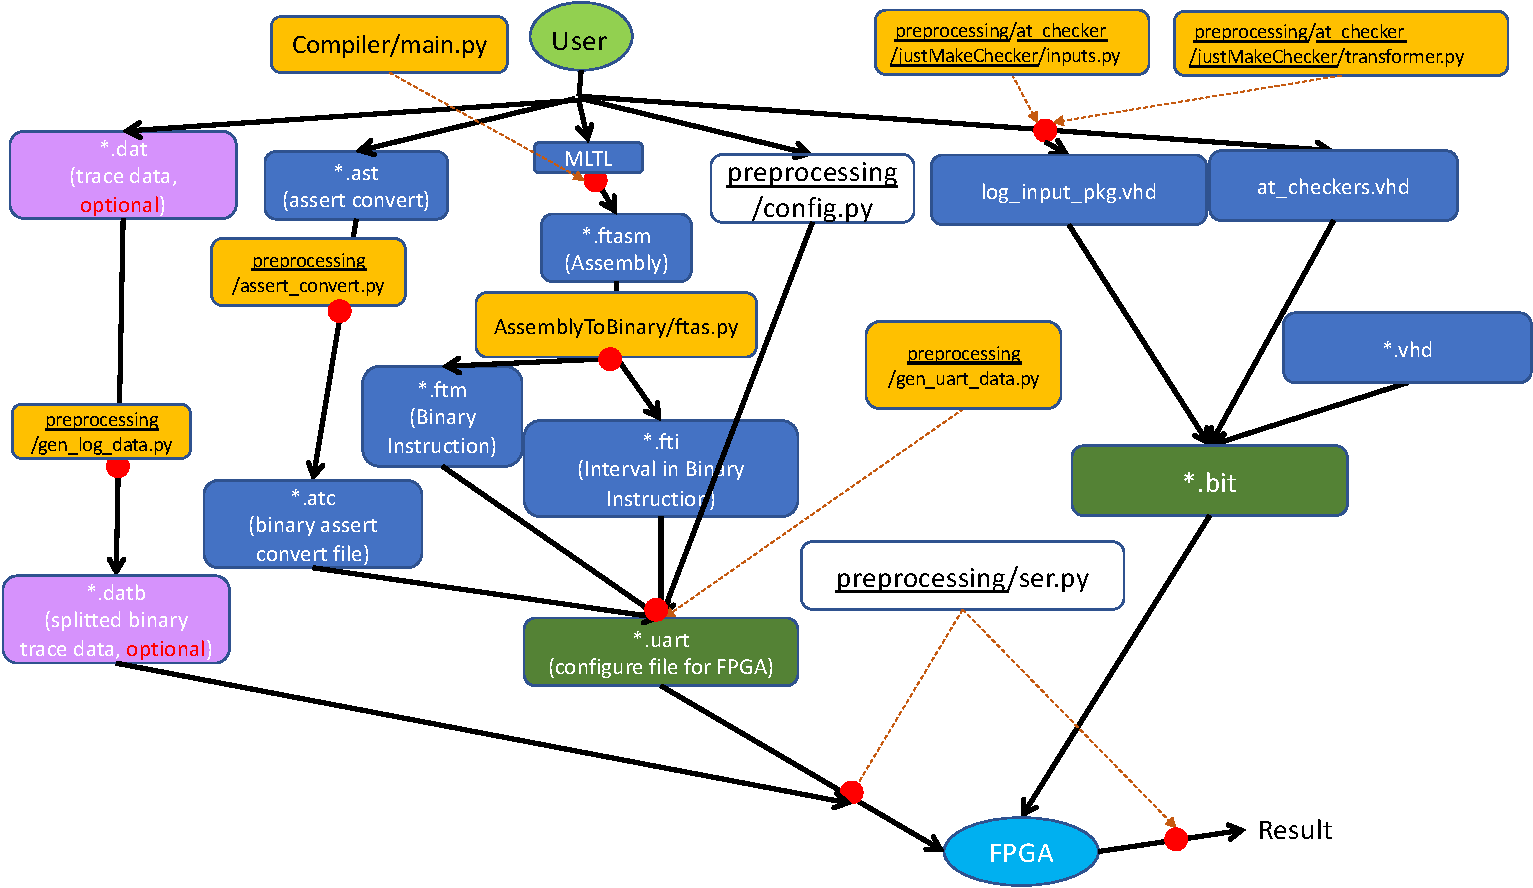
\includegraphics[scale=0.5]{fig/r2u2_fpga_flow.pdf}
	\caption{The flow of how the VHDL version of R2U2 is compiled and deployed. 
	\label{fig:r2u2hwFlow}} 
	\end{center}
\end{figure}

\subsection{User Specified Files}
This section describes the different files users need to provide or modify to launch the hardware version of R2U2. 
\subsubsection{Configuration File}
\label{config}
The first step is to tailor the \textit{config.py} file (located within the \textbf{../tools/preprocessing} directory) for the specific project. The following parameters can be modified within this file:
\begin{itemize}
	\item \textbf{SENSOR\_DATA\_WIDTH:} The maximum number of bits in the input to the atomic checkers. The upper-bound of this parameter is 32-bits.
	\item \textbf{NUM\_OF\_SENSOR:} The number of sensor inputs interfacing with R2U2.
	\item \textbf{SERIAL\_RUN\_MODE:} The mode in which R2U2 will execute.
	\begin{itemize}
		\item \textbf{self\_sensing:} R2U2 will execute based on the sensor input values streamed from external hardware.
		\item \textbf{read\_log:} R2U2 will execute based on the trace file given in \textbf{SENSOR\_DATA\_FILE}.
		\item \textbf{type\_input:} R2U2 will execute based on the binary values transmitted via the CLI.
	\end{itemize}
	\item \textbf{DATA\_SAMPLE\_NUMBER:} The number of time stamps R2U2 will execute across a \textbf{read\_log} trace.
\end{itemize}

\subsubsection{MLTL Formula}
\label{HWmltlFormula}
The MLTL formula that R2U2 will reason over must be implemented in one of two ways: either written and saved into the \textit{main.py} file (located within the \textbf{tools/Compiler} directory) or entered directly into the CLI when compiling the \textit{.ftasm} assembly file. In either case the syntax for the MLTL formula is identical and an example of an MLTL formula is shown in Table \ref{HWmltlFormulaTable}. Note that the only difference is how special characters are labeled in the CLI: they must be proceeded with a `` $\setminus$ ''. Additionally, the syntax for the MLTL formulas can be seen in Table \ref{HWsyntaxMLTL}.

\begin{table}[H]
	\caption{An example of an MLTL formula and the syntactical conversion into either the file type or the CLI.}
	\label{HWmltlFormulaTable}
	\begin{center}
	\begin{tabular}{l | l}
		\hline
		\hline
		\textbf{Type} & \textbf{Formula Format}\\
		\hline
		Expression & $G_{0,3}((a_0\bigwedge a_1)\bigwedge (a_2 \bigwedge s_3))$\\
		\textit{main.py} & MLTL = ``G[0,3]((a0 \& a1) \& (a2 \& a3))''\\
		CLI & G[0,3]((a0$\setminus$\&a1) $\setminus$\&(a2$\setminus$\&a3))\\
		\hline
		\hline
	\end{tabular}
	\end{center}
\end{table}

\begin{table}[H]
	\caption{The format for the MLTL operators, which are used to create a single MLTL formula which can either be saved to the \textit{main.py} file or incorporated into the CLI. Note that $E$1 and $E$2 denote that that parameter can be either a single atomic or an expression, to allow for more complex formulas.}
	\label{HWsyntaxMLTL}

	\begin{center}
	\begin{tabular}{l | c | c | c | c | c | c}
		\hline
		\hline
		\textbf{Expression} & \textit{NOT} & \textit{Next} & \textit{Until} & \textit{Global} & \textit{AND} & \textit{OR}\\
		\hline
		\textbf{Syntax} & !$E$1 & $XE$1 & $E$1 $U$[$t_i$,$t_f$] $E$2 & $G$[$t_i$,$t_f$] $E$1 & $E$1 \& $E$2& $E$1 $|$ $E$2\\
		\hline
		\textbf{Precedence} & 1 & 1 & 2 & 2 & 3 & 3\\
		\hline
		\hline
	\end{tabular}
	\end{center}
\end{table}

\subsubsection{Configuring Atomic Checkers}
\label{ConfigAC}

\subparagraph{Atomic Checker File:}
Since R2U2 reasons over Boolean values, sensor values must be pre-processed into Boolean atomics. This is done by R2U2's Atomic Checkers, which can perform fixed-point addition, subtraction, and a power-of-two multiplication/division on no more than two sensor values. Then it performs a comparison operation against a predefined value, to determine its Boolean output.

Each atomic in R2U2's MLTL formula will have its own Atomic Checker Block in hardware. The \textit{inputs.py} script in the \textbf{tools/preprocessing} directory allows users to specify the bit-length, name, and units of their sensor signals. From there, the \textit{transformer.py} script can be executed to automatically generate the VHDL file for R2U2 with the specified number of atomic checker blocks.

\subparagraph{Atomic Checker Block:}
The hardware for an atomic checker block must be customized for each instantiation. within the design. A diagram for this hardware block can be seen in Fig. \ref{fig:ACB}.

\begin{figure}[H]
	\begin{center}
	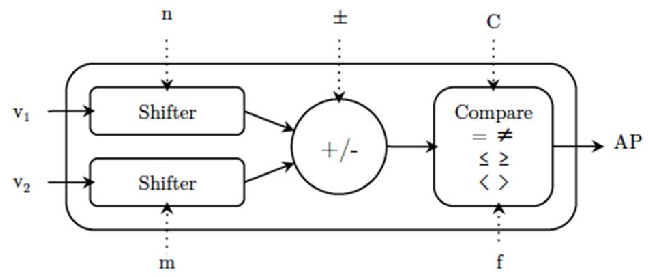
\includegraphics[scale=0.5]{fig/AtomicCheckerBlock.pdf}
	\caption{A high-level schematic of the configurable Atomic Checker block.
	\label{fig:ACB}} 
	\end{center}
\end{figure}

To configure each checker within the design, the user must modify the \textit{input.ast} file within the \textbf{tools/preprocessing} directory. In this file, each line indicates the configuration for each atomic checker. The syntax for this file reads as follows:

\begin{equation}
	C;n;m;Op;F
\end{equation} 
where $C$ is the integer value used in the comparison, $n$ \& $m$ are the number of arithmetic shifts performed on $v_1$ \& $v_2$, respectively, $Op$ is the mathematical operation performed on the post-shifted input values, and $F$ is the selected comparison function for the block. The syntax for the comparison \& arithmetic operations can be seen in Table \ref{syntaxACB}. Note that the shift operations can be used to perform fixed-point multiplication or division by powers of 2. 

\begin{table}[H]
	\caption{The valid comparison \& arithmetic operations the Atomic Checker block can perform as well as their respective syntax for the \textit{input.ast} file.
	\label{syntaxACB}}
	\begin{center}
	\begin{tabular}{l | c | c | c | c | c | c}
		\hline
		\hline
		&\multicolumn{6}{c}{\textbf{Comparison Operations}}\\
		\hline
		\textbf{Operation} & $=$ & $\neq$ & $\geq$ & $>$ & $\leq$ & $<$ \\
		\hline
		\textbf{Syntax} & \textit{EQU} & \textit{NEQ} & \textit{GEQ} & \textit{GRE} & \textit{LEQ} & \textit{LES}\\
		\hline
		\hline
		&\multicolumn{6}{c}{\textbf{Arithmetic Operations}}\\
		\hline
		\textbf{Operation} & \multicolumn{2}{c}{$v_1+v_2$} & \multicolumn{2}{c}{$v_1-v_2$} &\multicolumn{2}{c}{$|v_1-v_2|$} \\
		\hline
		\textbf{Syntax} & \multicolumn{2}{c}{\textit{ADD}} & \multicolumn{2}{c}{\textit{SUB}} & \multicolumn{2}{c}{\textit{DIF}}\\
		\hline
		\hline
	\end{tabular}
	\end{center}
\end{table}

After configuring the \textit{input.ast} file for the given project, execute the script \textit{assert\_convert.py} script to automatically convert the configurations within the \textit{input.ast} file into a binary format suitable for the hardware.


\subsubsection{Modifying the VHDL Files}
\label{ModVHDL}
This section describes R2U2's VHDL files that a user would need to modify for their own sensors to be integrated with the hardware version of R2U2. The atomic checker blocks of R2U2 are configurable for up to a 32-bit fixed-point value. Thus, the sensor data must be passed to R2U2 as a fixed-point value. This can be done by connecting R2U2 directly to a software configurable register or a custom hardware preprocessing component. Note that a basic outline for interfacing R2U2 with a custom hardware component is given, but there may be additional modifications necessary for interfacing software registers to R2U2, i.e., additional files for interfacing with the CPU via AXI to allow for software configurable registers to hold sensor values.

\subparagraph{sensor\_log.vhd:} The \textit{sensor\_log.vhd} file (in the \textbf{R2U2\_HW/customize} directory) must be customized for the desired project. Note that this is where R2U2 registers the incoming sensor data and stores it into a singular register \textit{\textbf{log\_data}} of \textbf{LOG\_DATA\_WIDTH}, which is a concatenation of the one or more sensor's fixed-point data. Currently, R2U2's \textit{\textbf{log\_data}} register stores the sensors in descending order, with the order specified in the \textit{inputs.py} file (in the \textbf{tools/preprocessing} directory). 

\begin{figure}[H]
	\begin{center}
	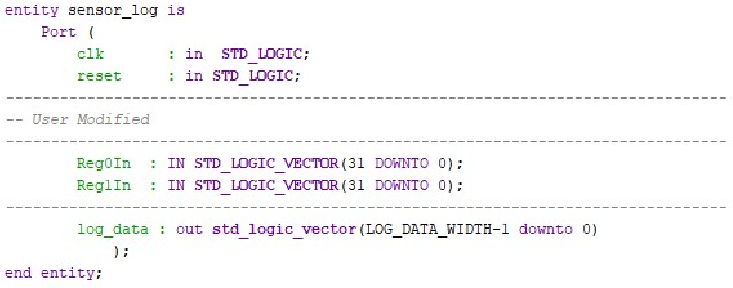
\includegraphics[scale=0.5]{fig/r2u2_hw_sensorLog_entity.pdf}
	\caption{A screenshot of \textit{sensor\_log.vhd}'s entity block, showing where the user will configure the file's input parameters. 
	\label{fig:r2u2hwSLentity}} 
	\end{center}
\end{figure}

\begin{figure}[H]
	\begin{center}
	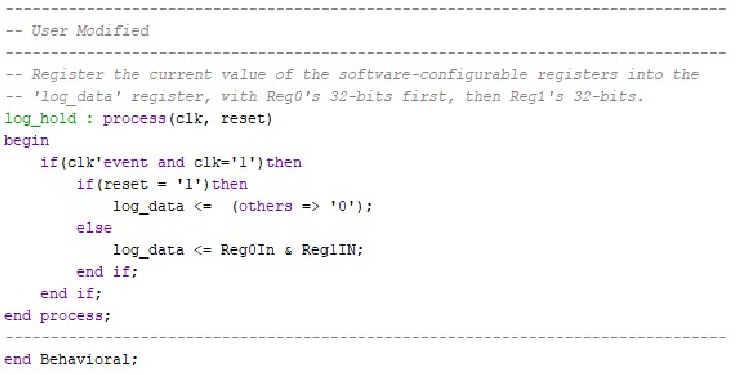
\includegraphics[scale=0.5]{fig/r2u2_hw_sensorLog_arch.pdf}
	\caption{A screenshot of \textit{sensor\_log.vhd}'s architecture block, showing where the user will configure the file's process block so that the \textit{\textbf{log\_data}} register is the concatenation of all the sensor values. 
	\label{fig:r2u2hwSLarch}} 
	\end{center}
\end{figure}

\subparagraph{echo.vhd:} The file \textit{echo.vhd} (located in the \textbf{R2U2\_HW/uart} directory) instantiates the file \textit{sensor\_log.vhd}. Thus, we must modify this file, specifically its entity block, the component declaration, and the component instantiation, as seen in Fig. \ref{fig:r2u2hwEchoEnt}, \ref{fig:r2u2hwEchoCom}, and \ref{fig:r2u2hwEchoInst}.

\begin{figure}[H]
	\begin{center}
	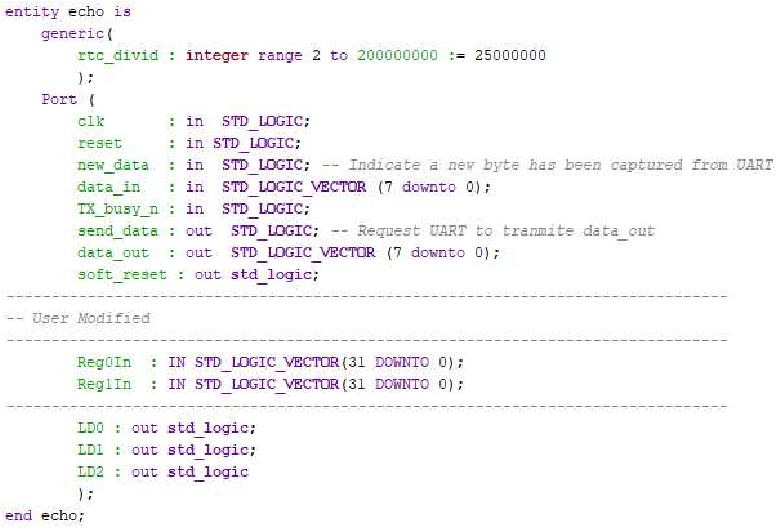
\includegraphics[scale=0.5]{fig/r2u2_hw_echo_entity.pdf}
	\caption{A screenshot of \textit{echo.vhd}'s entity block, showing where the user will configure the file's inputs to match those of \textit{sensor\_log.vhd}
	\label{fig:r2u2hwEchoEnt}} 
	\end{center}
\end{figure}

\begin{figure}[H]
	\begin{center}
	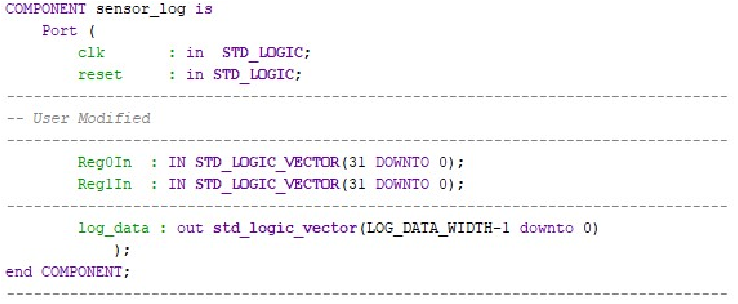
\includegraphics[scale=0.5]{fig/r2u2_hw_echo_component.pdf}
	\caption{A screenshot of \textit{echo.vhd}'s component declaration, showing where the user will configure the \textbf{sensor\_log} component's input signals to match those of the \textit{sensor\_log.vhd}'s entity block.
	\label{fig:r2u2hwEchoCom}} 
	\end{center}
\end{figure}

\begin{figure}[H]
	\begin{center}
	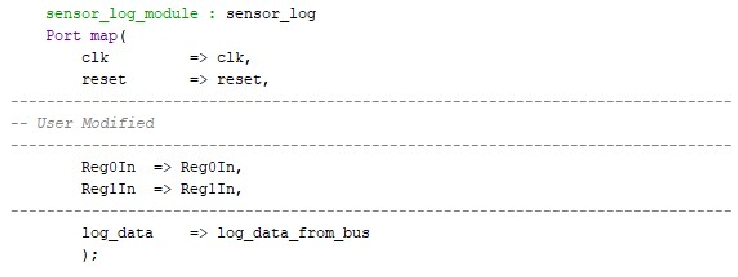
\includegraphics[scale=0.5]{fig/r2u2_hw_echo_inst.pdf}
	\caption{A screenshot of \textit{echo.vhd}'s instantiation of the \textbf{sensor\_log}, showing where the user will configure the signals to match those within their current design.
	\label{fig:r2u2hwEchoInst}} 
	\end{center}
\end{figure}

\subparagraph{process\_data.vhd:} The file \textit{process\_data.vhd} (located in the \textbf{R2U2\_HW/uart} directory) instantiates the file \textit{echo.vhd}. Thus, we must modify this file, specifically its entity block, the component declaration, and the component instatiation, as seen in Fig. \ref{fig:r2u2hwProEnt}, \ref{fig:r2u2hwProCom}, and \ref{fig:r2u2hwProInst}.

\begin{figure}[H]
	\begin{center}
	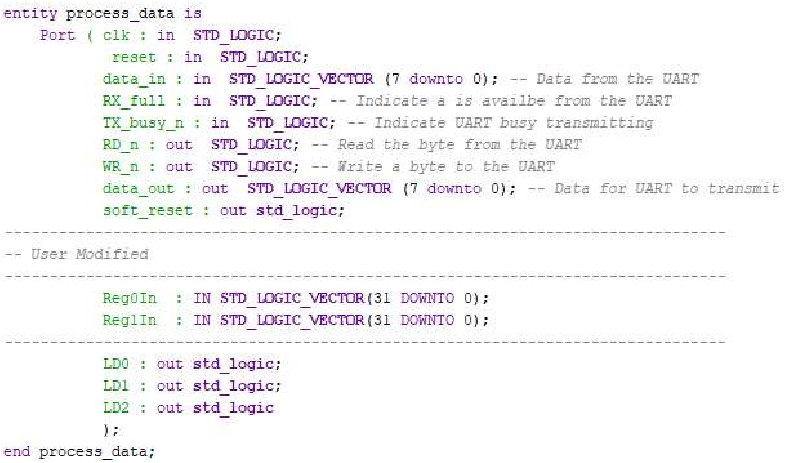
\includegraphics[scale=0.5]{fig/r2u2_hw_process_entity.pdf}
	\caption{A screenshot of \textit{process\_data.vhd}'s entity block, showing where the user will configure the file's inputs to match those of \textit{echo.vhd}
	\label{fig:r2u2hwProEnt}} 
	\end{center}
\end{figure}

\begin{figure}[H]
	\begin{center}
	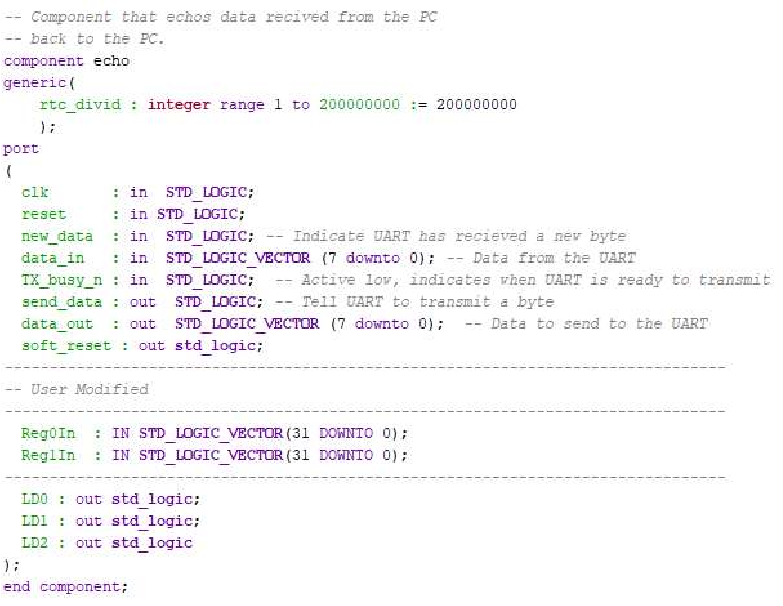
\includegraphics[scale=0.5]{fig/r2u2_hw_process_component.pdf}
	\caption{A screenshot of \textit{process\_data.vhd}'s component declaration, showing where the user will configure the \textbf{echo} component's input signals to match those of the \textit{echo.vhd}'s entity block.
	\label{fig:r2u2hwProCom}} 
	\end{center}
\end{figure}

\begin{figure}[H]
	\begin{center}
	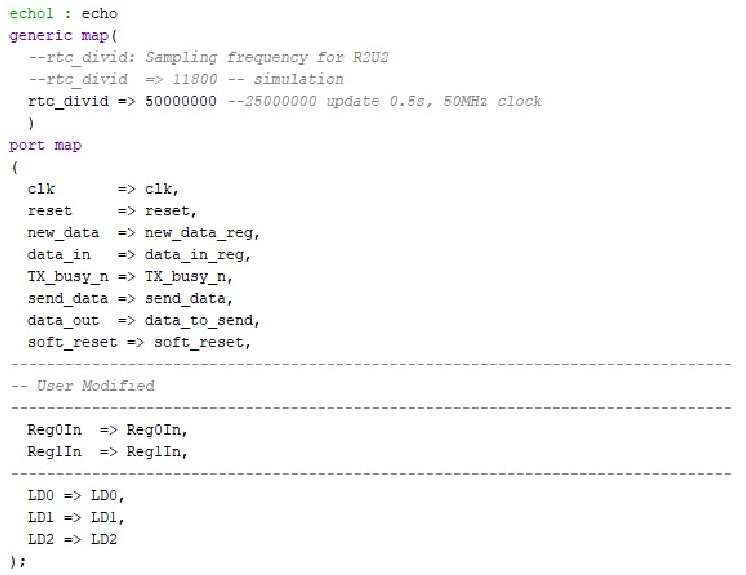
\includegraphics[scale=0.5]{fig/r2u2_hw_process_inst.pdf}
	\caption{A screenshot of \textit{process\_data.vhd}'s instantiation of the \textbf{echo}, showing where the user will configure the signals to match those within their current design.
	\label{fig:r2u2hwProInst}} 
	\end{center}
\end{figure}

\subparagraph{MP1.vhd:} The file \textit{MP1.vhd} (located in the \textbf{R2U2\_HW/uart} directory) is the top-level file for the design, i.e., this file connects all the other relevant files for the hardware version of R2U2. Thus, this file instantiates both the \textit{process\_data.vhd} file and the user's custom hardware file. Thus, we must modifty its entity block, the component declarations, the signal declarations, and the component instantiations, as seen in Fig. \ref{fig:r2u2hwMP1Ent}, \ref{fig:r2u2hwMP1Comp}, \ref{fig:r2u2hwMP1customComp}, \ref{fig:r2u2hwMP1customSig}, \ref{fig:r2u2hwMP1Inst}, and \ref{fig:r2u2hwMP1customInst}. 

\begin{figure}[H]
	\begin{center}
	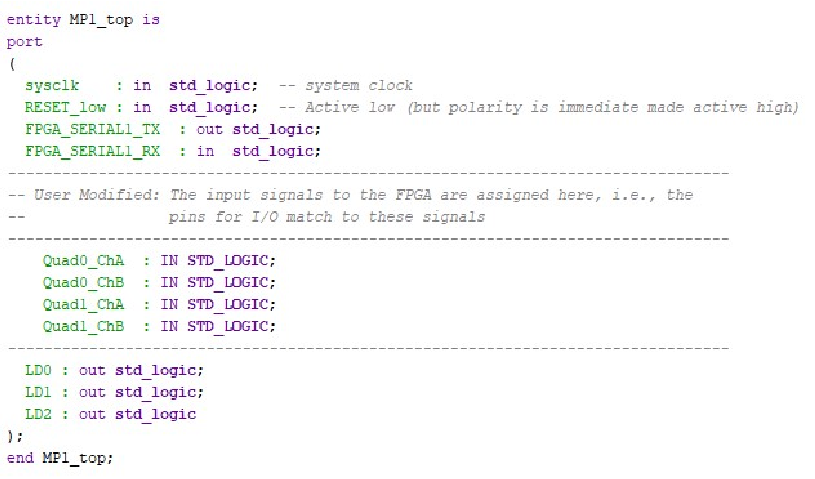
\includegraphics[scale=0.5]{fig/r2u2_hw_mp1_entity.pdf}
	\caption{A screenshot of \textit{MP1.vhd}'s entity block, showing where the user will configure the file's inputs from the FPGA's pins.
	\label{fig:r2u2hwMP1Ent}} 
	\end{center}
\end{figure}

\begin{figure}[H]
	\begin{center}
	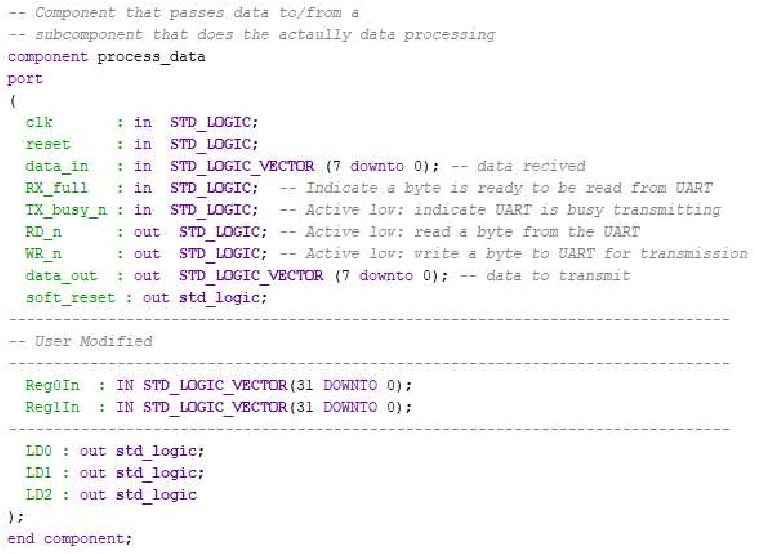
\includegraphics[scale=0.5]{fig/r2u2_hw_mp1_component.pdf}
	\caption{A screenshot of \textit{process\_data.vhd}'s component declaration, showing where the user will configure the \textbf{process\_data} component's input signals to match those of the \textit{process\_data.vhd}'s entity block.
	\label{fig:r2u2hwMP1Comp}} 
	\end{center}
\end{figure}

\begin{figure}[H]
	\begin{center}
	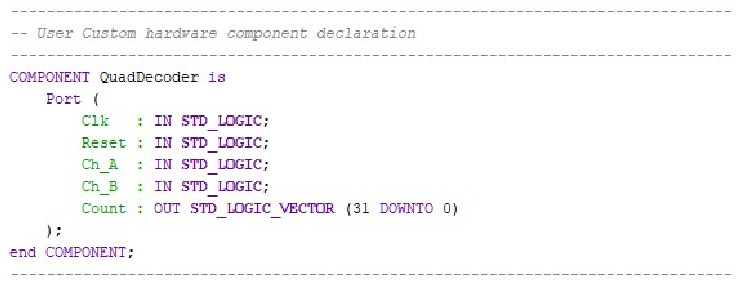
\includegraphics[scale=0.5]{fig/r2u2_hw_mp1_custom_comp.pdf}
	\caption{A screenshot of a custom hardware's component declaration.
	\label{fig:r2u2hwMP1customComp}} 
	\end{center}
\end{figure}

\begin{figure}[H]
	\begin{center}
	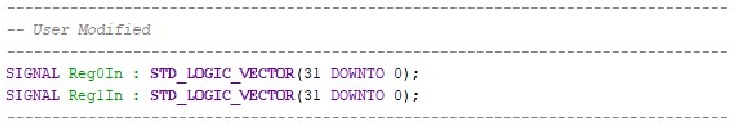
\includegraphics[scale=0.5]{fig/r2u2_hw_mp1_custom_signals.pdf}
	\caption{A screenshot of the custom signals \textbf{Reg0In} and \textbf{Reg1In}, which must be declared inside \textbf{MP1}'s architecture block to connect the instantiations of the custom hardware to the \textbf{process\_data} instantiation.
	\label{fig:r2u2hwMP1customSig}} 
	\end{center}
\end{figure}

\begin{figure}[H]
	\begin{center}
	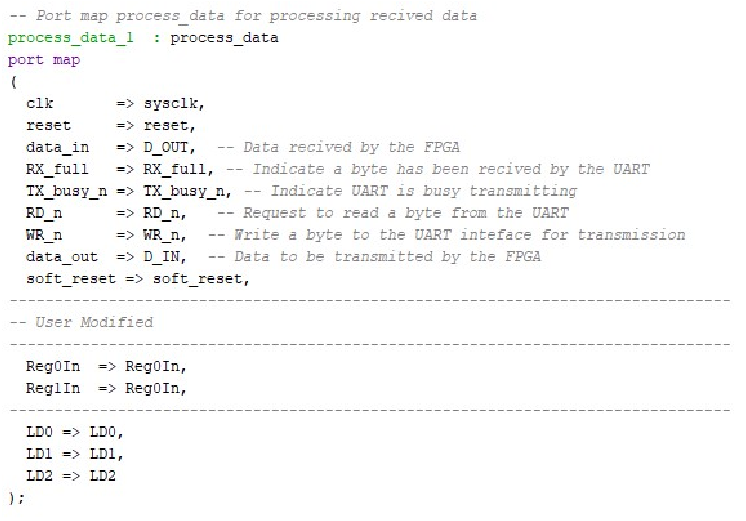
\includegraphics[scale=0.5]{fig/r2u2_hw_mp1_inst.pdf}
	\caption{A screenshot of \textit{MP1.vhd}'s instantiation of the \textbf{process\_data}, showing where the user will configure the signals to match those within their current design.
	\label{fig:r2u2hwMP1Inst}} 
	\end{center}
\end{figure}

\begin{figure}[H]
	\begin{center}
	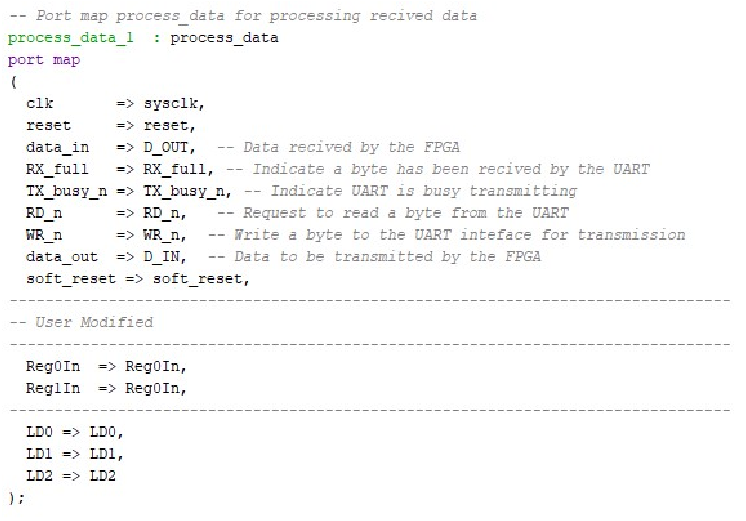
\includegraphics[scale=0.5]{fig/r2u2_hw_mp1_custom_inst.pdf}
	\caption{A screenshot of \textit{MP1.vhd}'s instantiation of the custom hardware, showing where the user will configure the signals to match those within their current design.
	\label{fig:r2u2hwMP1customInst}} 
	\end{center}
\end{figure}

\subsection{Running R2U2-VHDL}
\label{runR2U2}
\begin{enumerate}
% ***** Step #1 ***** 
	\item Navigate to the \textbf{tools/preprocessing} directory via
	\begin{lstlisting}[language=C]
	cd tools/preprocessing/
	\end{lstlisting}
	
% ***** Step #2 *****
	\item Modify \textit{config.py} file (refer to Section \ref{config}). Once modified to the desired settings, execute \textit{config.py} via:
	\begin{lstlisting}[language=C]
	python config.py
	\end{lstlisting}
	
% ***** Step #3 *****
	\item Navigate to the \textbf{tools} directory via:
	\begin{lstlisting}[language=C]
	cd ../
	\end{lstlisting}
	
% ***** Step #4 *****
	\item Modify \textit{main.py} in the \textbf{/tools/Compiler} directory with the desired MLTL formula. Note that the syntax for the MLTL formula must match that in Section \ref{HWmltlFormula}.
	
% ***** Step #5 *****
	\item Once the desired MLTL formula is in the \textit{main.py} file, convert the formula into the \textit{.ftasm} \& \textit{.ftscq} file structure via:
	\begin{lstlisting}[language=C]
	python Complier/main.py
	\end{lstlisting}
	
% ***** Step #6 *****
	\item Convert the \textit{.ftasm} assembly MLTL formula into the binary assembly \textit{.ftm} and binary assembly interval \textit{.fti} file structures via: 
	\begin{lstlisting}[language=C]
	cat tmp.ftasm | AssemblyToBinary/ftas.py tmp
	\end{lstlisting}
	
% ***** Step #7 *****
	\item Naviagate to the \textbf{preprocessing/at\_checker} directory via: 
	\begin{lstlisting}[language=C]
	cd preprocessing/at_checker
	\end{lstlisting}
	
% ***** Step #8 *****
	\item Modify the \textit{inputs.py} script to  the correct number \& bit-length of sensor inputs and create the correct number of atomic checker blocks. Run the \textit{transformer.py} script via: 
	\begin{lstlisting}[language=C]
	python transformer.py
	\end{lstlisting}
	
% ***** Step #9 *****
	\item Navigate back to the \textbf{tools/preprocessing} directory via: 
	\begin{lstlisting}[language=C]
	cd ../
	\end{lstlisting}
	
% ***** Step #10 *****
	\item Copy the \textit{at\_checkers.vhd} and \textit{log\_input\_pkg.vhd} files into the \textbf{R2U2\_HW/customize} directory via:
	\begin{lstlisting}[language=C]
	cp at_checkers.vhd log_input_pkg.vhd ../../../R2U2_HW/customize
	\end{lstlisting}
% ***** Step #11 *****
	\item Within the \textbf{tools/preprocessing} directory, modify the \textit{input.ast} file with the correct configurations for each atomic checker block. 

% ***** Step #12 *****
	\item Convert the \textit{input.ast} file into the \textit{res.atc} file via: 
	\begin{lstlisting}[language=C]
	python assert_convert.py
	\end{lstlisting}
	
% ***** Step #13 *****
	\item Within the \textbf{/R2U2\_HW/customize} directory, modify the \textit{sensor\_log.vhd} file to store the sensor values within the its \textit{log\_data} output register (as seen in Section \ref{ModVHDL}).
	
% ***** Step #14 *****
	\item Launch Vivado and create a new project. Import the \textbf{R2U2\_HW} directory  as the source file, create a constraint file for the user's board (example one - \textit{zybo.xdc} - is shown in the \textbf{R2U2\_HW/customize} directory), and choose the correct development board or FPGA (example one is the Zybo with the xc7z010 FPGA). In the \textbf{Sources} tab, set \textit{UART\_HW:MP1\_top} as the top-level file. Then synthesize \& generate the project's bitstream. Program R2U2 onto the FPGA.
	
% ***** Step #15 *****
	\item If using the \textbf{online mode} (\textbf{SERIAL\_RUN\_MODE:} self\_sensing), skip to next step. Else, if using \textbf{offline mode} (\textbf{SERIAL\_RUN\_MODE:} read\_log):
	\begin{enumerate}
		\item Modify \textit{sensor\_data.dat} with the sensor trace
		\item Convert the \textit{sensor\_data.dat} to a binary version the UART can transmit via:
	\begin{lstlisting}[language=C]
	python gen_log_data
	\end{lstlisting}
	\end{enumerate}


% ***** Step #16 *****
	\item Merge the \textit{.atc}, \textit{.ftm}, and \textit{.fti} files together into the \textit{.uart} file structure via: 
	\begin{lstlisting}[language=C]
	python gen_uart_data
	\end{lstlisting}

% ***** Step #16 *****
	\item From the \textbf{/tools/preprocessing} directory, launch a serial connection to the external serial-to-UART connection via: 
	\begin{lstlisting}[language=C]
	python ser.py
	\end{lstlisting}
	Note that this command must be launched using Version 2 of Python. It will not execute in Python 3.
	
\end{enumerate}

\clearpage

\section{R2U2 Software Implementation in Python}
While R2U2 is designed to be an online, embedded runtime monitor, it can often be useful to verify a trace offline. The Python implementation of R2U2 allows one to use R2U2's verification abilities offline as a fast and efficient way to verify a trace or validate an atomic formula over a trace.

\subsection{Getting Started}
Note that the following must be installed in order to use the Python implementation of R2U2:
\begin{itemize}
	\item Python 3.6 (or greater)
	\item \textbf{Python Packages:} argparse, py, random, logging, sys, collections
\end{itemize}
The Python implementation of R2U2 also runs from a UNIX based command line interface (CLI). Additionally, there are several types of input files users may use: 
\begin{itemize}
	\item \textbf{Input File:} There are two options for this input: an \textit{Assembly File} or a \textit{MLTL Formula}. The details and an example of each these formats will be discussed in Section \ref{InputFiles}.
	\item \textbf{Trace File:} There are two formats that this version of R2U2 will accept: a \textit{Sensor Input File} or an \textit{Atomic Input File}. The details and an example of each of these formats will be discussed in Section \ref{TraceFiles}.
	\item \textbf{Output File:} The name of the output file from R2U2. Note that if this is left blank, the default output file's name will be \textit{untitled.txt}.
\end{itemize}

\subsection{File Formats}
Note that user must provide an Input File and a Trace File to run R2U2, though there is no restrictions on the combination of these files. The Input File specifies the temporal logic formulas over which the atomic propositions are reasoned over. The Trace File is the atomics or sensor values that are being reasoned over.

\subsubsection{Input File Formats}
\label{InputFiles}
There are two different formats in which the temporal logic formulas can be entered into the Python version of R2U2: (1) \textbf{Assembly File} or (2) \textbf{MLTL Formula}.

\subparagraph{Assembly File:}
\label{AssemblyFile}
Like any other assembly file, this file is a list of single command instructions that R2U2 will execute, in order. An example of a R2U2 compatible Assembly File can be seen in Table \ref{FileTable}. Each line contains an instruction, which consists of a label, a command, and one or more variables/labels. The list of assembly commands the Python version of R2U2 can use is:
\begin{itemize}
	\item \textbf{\textit{load}:} Used to load the atomic from either the Sensor Input File or Atomic Input File. 
	\item \textbf{\textit{not}:} Used to denote the logical \textit{Negation} of an atomic.
	\item \textbf{\textit{and}:} Used to denote the logical \textit{AND} of two atomics.
	\item \textbf{\textit{until}:} Used to denote the \textit{Until} temporal logic function. This function takes in four arguments: the first is the label for the left-side of the \textit{Until}, the second is the right-side, the third is the relative start time, and the fourth is the relative end time.
	\item \textbf{\textit{boxbox}:} Used to denote the \textit{Global} temporal logic function. Assumes that the time bound starts at zero. First argument is the label (either atomic or instruction), the second is the relative end time of the function.
	\item \textbf{\textit{boxdot}:} Used to denote the \textit{Global} temporal logic function. First argument is the label (either atomic or instruction), the second is the relative start time of the function, and the third is the relative end time of the function.
	\item \textbf{\textit{end}:} Used to denote the end of the assembly file. This command must be at the end of the Assembly File and its argument must be the second-to-last label.
\end{itemize}

\begin{table}[H]
	\caption{Examples of the format for the Input Files}
	\label{FileTable}
	\begin{center}
	\begin{tabular}{l | l}
		\hline
		\hline
		\textbf{File Type} & \textbf{Assembly File}\\
		\hline
		line 1 & s0: load a0\\
		line 2 & s1: load a1\\
		line 3 & s2: not a0\\
		line 4 & s3: not a1\\
		line 5 & s4: and a0 a1\\
		line 6 & s5: and s2 s3\\
		line 7 & s6: not s5\\
		line 8 & s7: until s7 s5 0 3\\
		line 9 & s8: boxbox s8 3\\
		line 10 & s9: end s8\\
		\hline
		\hline
	\end{tabular}
	\end{center}
\end{table}

\subparagraph{MLTL File:}
\label{MLTLFile}
When one, complex function is to be evaluated, a user may find it easier to generate a MLTL File, or enter the function directly via the CLI, rather than manually create the assembly code. The valid expressions for an MLTL formula are given in Table \ref{MLTLCommands}.

\begin{table}[H]
	\caption{The format for the MLTL formulas, either in a single line of a text file or via the CLI. Note that $E$1 and $E$2 denote that that parameter can be either an expression, to allow for more complex formulas, or a single atomic.}
	\label{MLTLCommands}
	\begin{center}
	\begin{tabular}{l | c | c}
		\hline
		\hline
		\textbf{Expression} & \textbf{Syntax} & \textbf{Precedence} \\
		\hline
		\textit{NOT} & !$E$1 & 1\\
		\textit{Next} & $XE$1 & 1\\
		\textit{Until} & $E$1 $U$[$t_i$,$t_f$] $E$2 & 2\\
		\textit{Until} & $E$1 $U$[$t_f$] $E$2 & 2\\
		\textit{Global} & $G$[$t_i$,$t_f$] $E$1 & 2\\
		\textit{Global} & $G$[$t_f$] $E$1 & 2\\
		\textit{AND} & $E$1 \& $E$2 & 3\\
		\textit{OR} & $E$1 $|$ $E$2 & 3\\
		\hline
		\hline
	\end{tabular}
	\end{center}
\end{table}

Note that precedence can be overruled using parenthesis or brackets. Additionally all tuple time stamps must be comma separated. The following is an example of a complex MLTL formula and its syntactical conversion into a command that the Python version of R2U2 can reason over:

\begin{equation}
G_{0,5}(\neg{a_0}U_{0,3} (a_1 \bigwedge a_2)) \bigvee \neg{Xa_0} \rightarrow ((G[5] ((!a0) U[0,3] (a1 \& a2))) | !(Xa0)
\label{ExampleMLTL}
\end{equation}

\subsubsection{Trace File Formats}
\label{TraceFiles}
The two Trace File formats are given in Table \ref{SensorFileTable}. Note that the two formats require the first line to be a label, either that of the sensor or the atomic. In order for the tool to parse the input file,  values in this file must be separated by a space or a comma. Each line is an increment in time, starting at time $t=0$.

\subparagraph{Sensor Input File:}
\label{SensorInputFile}
The values of the sensor input file can be either signed/unsigned integers, single/double precision floating point, or hexadecimal values. Since R2U2 reasons over boolean values, these sensor values must be converted to a boolean value by performing some type of conditional reasoning, i.e., $=$, $\neq$, $>$, $<$, $\geq$, $\leq$. To do this, the \textit{Traverse.py} file, located in the \textbf{R2U2\_SW/R2U2\_PYTHON/ACOW} directory, must be modified. Specifically the \textbf{def s2a} function maps the sensor functions into boolean atomics. Note that Fig.\ref{fig:sa} shows the formatting for how to perform the boolean mapping.
\begin{center}
	\begin{figure}[H]
		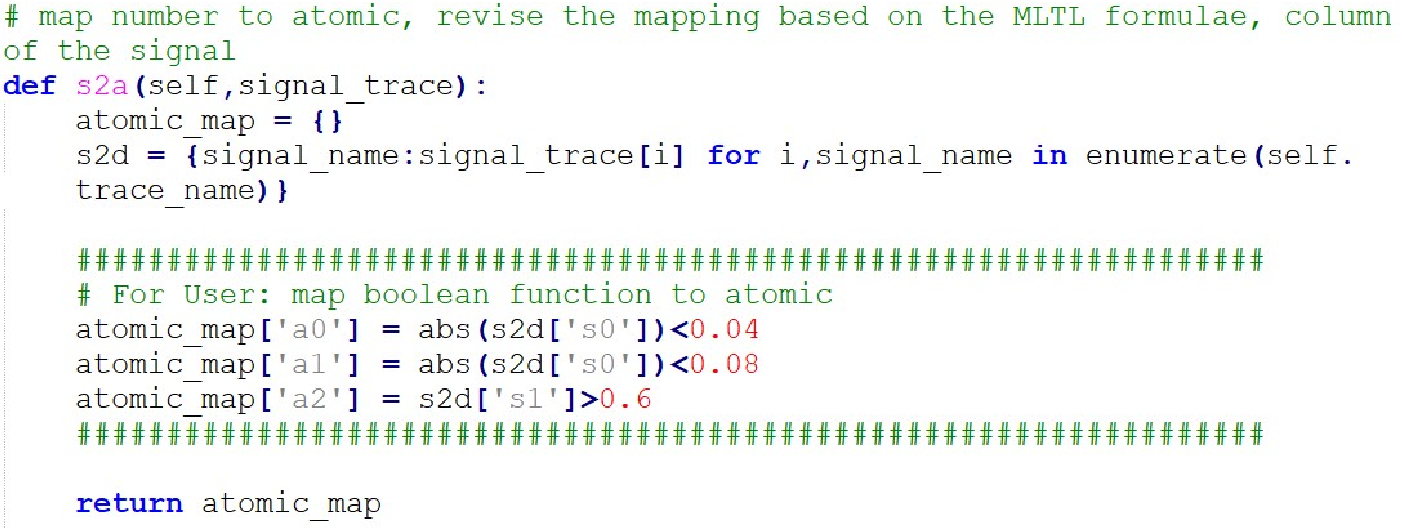
\includegraphics[scale=0.5]{fig/TraverseScreenshot.pdf}
		\caption{A screenshot of the \textbf{s2a} function within the \textit{Traverse.py} file. Note that this function must be modified in order to convert the sensor values into boolean atomics.}
		\label{fig:sa}
	\end{figure}
\end{center}

\subparagraph{Atomic Input File:}
\label{AtomicInputFile}
The values of the atomic input file must be Booleans, i.e., a $0$ or $1$. Unlike the sensor input file, there is no need to modify the \textit{Traverse.py} file when using this version of an input file. An example of the format can be seen in Table \ref{SensorTable}.

\begin{table}[H]
	\caption{Examples of the format for the Trace Files}
	\label{SensorTable}
	\begin{center}
	\begin{tabular}{l | ccc | ccc}
		\hline
		\hline
		\textbf{File Type} & \multicolumn{3}{c|}{\textbf{Sensor Input File}} & \multicolumn{3}{c}{\textbf{Atomic Input File}}\\
		\hline
		Line \# & Sensor 0 & Sensor 1 & $\dots$ & Atomic 0 & Atomic 1 & $\dots$\\
		\hline
		line 1 & Altitude & Velocity & $\dots$ & a0 & a1 & $\dots$\\
		line 2 & 1005 & 10.0 & $\dots$ & 0 & 0 & $\dots$\\
		line 3 & 1011 &  9.8 & $\dots$ & 1 & 0 & $\dots$\\
		line 4 & 1015 & 10.4 & $\dots$ & 1 & 1 & $\dots$\\
		line 5 & $\vdots$ & $\vdots$ & $\ddots$ & $\vdots$ & $\vdots$ & $\ddots$\\
		\hline
		\hline
	\end{tabular}
	\end{center}
\end{table}

\subsection{CLI Overview}
To use the Python version of R2U2, navigate to the \textbf{R2U2\_SW/R2U2\_PYTHON/} directory within a UNIX bash terminal. Verify your current version of Python by entering \textbf{python3 --version}. If your current version is Python 3.6 or greater, proceed. If not, you must install Python 3 to continue.

The command structure for running R2U2 is as follows:
\begin{lstlisting}[language=Bash]
	python MLTL_main.py -m "$(cat [A])" -s [B] -o [C]
\end{lstlisting}
where \textbf{[A]} is the path and name of Input File, \textbf{[B]} is the path and name of Trace File, and \textbf{[C]} is the name of the Output File. Remember that \textbf{[C]} is optional, and if it is not specified, then the default output file name is \textit{untitled.txt}. Note that if the user wishes to manually enter a MLTL formula into the command line, rather than use an input file, then the ``\$(cat [A])'' can be replaced with the MLTL formula.

\clearpage



\end{document}
